\documentclass[review]{elsarticle}

\usepackage{amsmath,amssymb,amsfonts}
\usepackage{algorithmic}
\usepackage{graphicx}
\usepackage{textcomp}
\usepackage{xcolor}
\usepackage{colortbl}
\usepackage[linesnumbered,ruled,vlined]{algorithm2e}
\usepackage{hyperref}
\usepackage{booktabs}
\usepackage{makecell}
\usepackage{multirow}
\usepackage{svg}
\usepackage{graphicx}
\usepackage{amsmath}
\usepackage{hyperref}
\usepackage{url}
\usepackage{booktabs}
\usepackage{amsfonts}
\usepackage{nicefrac}
\usepackage{microtype}
\usepackage{lipsum}
\usepackage{array}
\usepackage{multirow}
\usepackage{float}
\usepackage{natbib}
\usepackage{doi}
\usepackage[utf8]{inputenc}
\usepackage[T1]{fontenc}
\usepackage{hyperref}
\usepackage{amsmath}
\usepackage[table]{xcolor}
\definecolor{skyblue}{HTML}{5492C7}   % 天蓝
\definecolor{grass}{HTML}{99B86B}     % 浅草绿
\newcommand{\cont}{\ensuremath{^\mathsf{c}}}  % 一行放导言区
\usepackage[table]{xcolor}
\definecolor{lightgrass}{RGB}{153, 184, 107}
\definecolor{graywhite}{RGB}{231, 229, 223}


\bibliographystyle{elsarticle-num}

\makeatletter
\def\ps@pprintTitle{%
 \let\@oddhead\@empty
 \let\@evenhead\@empty
 \let\@oddfoot\@empty
 \let\@evenfoot\@empty
}
\makeatother

\begin{document}

\begin{frontmatter}


\title{DyCoT‑RE: Chain-of-Thought-Enhanced LLM Reward Engineering with Dual-Dynamic Optimization for Reinforcement Learning}

\author[shu]{Xinning Zhu}
\author[shu]{Jinxin Du}
\author[shu]{Longfei Huang}
\author[shu]{Lunde Chen\corref{cor1}}

\cortext[cor1]{Corresponding author\\Email: lundechen@shu.edu.cn}

\address[shu]{Sino-European School of Technology, Shanghai University, Shanghai, China}

\begin{abstract}
Designing effective reward functions remains a challenge in applying reinforcement learning (RL) to real-world tasks.
This paper proposes DyCoT-RE, a large language model (LLM)-driven reward engineering framework that integrates Chain-of-Thought (CoT) reasoningg with a dual-dynamic 
optimization strategy to automate and enhance reward function design.
The framework uses structured CoT reasoning iteratively generate and refine structured reward code.
It further incorporates a dual-dynamic optimization mechanism, 
comprising a temperature adjustment module that modulates the sampling temperature based on policy entropy trends, 
and a model switching module that dispatches language models with different capabilities to produce distinct reward components.
\textcolor{red}{Evaluations across four RL environments: CartPole, BipedalWalker, Ant, and SpaceMining. 
The latter is a novel environment, absent from standard RL benchmarks and LLMs pretraining corpora. }
DyCoT-RE consistently achieves higher average rewards and faster learning compared to human-designed and non-CoT baselines, as well as single-optimization variants.
These results demonstrate its potential as a scalable and adaptive solution for complex, evolving reward design.

\end{abstract}

\begin{keyword}
Reinforcement learning \sep reward engineering \sep large language models \sep chain-of-thought reasoning \sep dynamic temperature adjustment \sep model selection
\end{keyword}

\end{frontmatter}

\section{Introduction}

Reinforcement learning has achieved impressive results across diverse domains. 
\textcolor{red}{Indeed,} as Sutton et al. \cite{sutton1998reinforcement} emphasize, the reward signal is the primary means of specifying task objectives in RL, making its design critical to achieving desired behaviors.
In practice, translating intended behaviors into precise, effective reward functions remains highly challenging, particularly for tasks involving long-term dependencies 
\cite{amodei2016concrete}.
Skalse et al. \cite{skalse2022misspecification} demonstrate that agents often exploit imperfections in reward formulations to maximize proxy objectives in unintended ways, leading to behaviors that optimize the designed reward but undermine true task performance.
These challenges suggest that although reinforcement learning offers strong theoretical flexibility, its real-world applications are frequently limited by the complexity and domain-specific knowledge required to design effective reward functions. \cite{ibarz2018reward}.

While carefully designed rewards can accelerate agent learning and improve task performance,
manual reward engineering typically relies on trial-and-error tuning,
which is labor-intensive and often yields suboptimal generalization to new environments or objectives \cite{hadfield2017inverse}.
As RL applications grow in complexity, there is a pressing need for methods that can automate
reward design while maintaining interpretability and flexibility.

Recent advances in LLMs have demonstrated strong reasoning and generalization capabilities \cite{brown2020language, ouyang2022training}.
In particular, CoT reasoning enables LLMs to decompose tasks into structured intermediate steps,
enhancing clarity and ensuring closer correspondence to intended objectives.
This structured reasoning process suggests a promising direction for reward engineering, 
as it provides a means of translating task descriptions into reward functions with well-defined objectives.

However, existing CoT-based reward generation approaches typically use static sampling parameters and fixed model configurations,
which may limit their adaptability.
Recent studies have emphasized the need for dynamic adaptation in LLM-based systems to improve sample efficiency and maintain adaptability to evolving task requirements.
For example, Nguyen et al. \cite{nguyen2024turning} demonstrate that min-p sampling enhances creativity while preserving coherence in narrative generation tasks, while Peeperkorn et al. \cite{peeperkorn2024temperature} analyze temperature as a direct modulator of LLM creativity.
Moreover, Fedus et al. \cite{fedus2022switch} and Du et al. \cite{du2022glam} show that mixture-of-experts architectures can scale model capacity efficiently via adaptive routing.
Collectively, these findings demonstrate that dynamic mechanisms such as temperature adjustment and expert model selection can enhance adaptability in LLM-driven systems.

In this work, we propose DyCoT-RE, a reward engineering framework that combines structured CoT reasoning
with dual-dynamic optimization.
Specifically, DyCoT-RE leverages CoT reasoning to decompose natural language task descriptions into structured reward components,
then employs iterative refinement to enhance alignment with intended task objectives.
\textcolor{red}{The dual-dynamic optimization strategy employs two mechanisms to support this process: 
entropy-guided temperature adjustment balances exploration and exploitation, 
while the dynamic model selection module routes sub-tasks to specialized LLMs based on performance feedback.
By coupling these components within a closed-loop evolutionary search process, 
DyCoT-RE facilitates systematic reward engineering and improves training efficiency in complex reinforcement learning tasks.}


We evaluate DyCoT-RE on the standard RL environments CartPole,
BipedalWalker, and Ant to assess its performance across different control tasks.
While these environments are widely used, recent studies have raised concerns that LLMs may possess latent knowledge about 
them from pretraining corpora, potentially leading to prompt leakage and evaluation bias\cite{huang2025thinkbench, qi2024quantifying, lu2024mental}. 
To address this concern and test DyCoT-RE’s adaptability to unfamiliar scenarios, we additionally introduce a custom-designed environment, 
SpaceMining\footnote{Project website: \url{https://reveurmichael.github.io/space_mining/}.}, which represents a novel task domain.
Experimental results show that DyCoT-RE consistently achieves higher average rewards 
and faster convergence than baseline and non-CoT methods across all evaluated environments.

The remainder of this paper is organized as follows.
Section 2 reviews related work in reward engineering, chain-of-thought reasoning, and dynamic optimization in LLM-based systems.
Section 3 introduces the DyCoT-RE framework, including CoT-based reward construction and the dual-dynamic optimization strategy.
Section 4 presents experimental evaluations, including setup, benchmark comparisons, ablations, and evaluation in a novel environment.
Section 5 discusses the main findings, limitations, and potential directions for future work.
Section 6 concludes the paper.



\section{Related Work}

\subsection{Reward Engineering Paradigms}

In RL, the design of effective reward functions directly shapes agent behavior and learning outcomes. 
Traditional approaches primarily rely on handcrafted reward functions informed by domain expertise. 
While intuitive, such manual design often struggles to capture complex, dynamic task objectives and is prone to 
suboptimal or biased formulations, hindering agent performance in real-world scenarios.

To address these limitations, reward shaping was introduced as a formal enhancement strategy. 
Ng et al. \cite{ng1999policy} demonstrated that potential-based reward shaping preserves optimal policies 
while enabling accelerated convergence, laying the theoretical foundation for numerous practical implementations. 
Intrinsic motivation frameworks further advanced this field by encouraging exploration through curiosity-driven signals. 
Singh et al. \cite{singh2010intrinsically} proposed intrinsic rewards to incentivize novel state visits, 
later extended by Burda et al. \cite{burda2018exploration}, who empirically validated large-scale curiosity-driven exploration 
benefits across diverse environments.

Despite these developments, manually designing rewards for complex or evolving tasks remains inefficient and costly. 
LLMs offer a promising alternative by leveraging their natural language understanding to automate reward generation 
and optimization. Unlike traditional RL pipelines that require explicit, task-specific reward formulations, 
LLMs can interpret high-level task descriptions, extract key objectives, and translate them into executable reward functions. 
This capability facilitates more intuitive alignment with human intentions, reduces engineering overhead, and enhances agent 
adaptability.

Recent studies have increasingly leveraged LLMs for automated reward engineering in reinforcement learning. 
Early demonstrations showed that language descriptions can serve as reward signals or be translated into executable reward code, 
notably Reward Design with Language Models \cite{kwon2023reward} and Language-to-Rewards (L2R) \cite{yu2023language}. 
Building on this concept, rapid progress has been made, from simple prompts to automatic code generation and closed-loop optimization.
Representative works include Text2Reward \cite{xie2023text2reward} for dense reward shaping with iterative refinement, 
VLM-based zero-shot rewards \cite{rocamonde2023vision} using vision-language models, and LLM4PG \cite{shen2024beyond} for automated 
preference labeling. 

Among these, Eureka \cite{ma2023eureka} demonstrates a notable automated framework that treats LLMs as autonomous agents, 
iteratively generating, mutating, and selecting reward code via performance-based tournaments.
In their evaluation, Eureka achieved performance improvements over expert-designed rewards across several RL tasks, 
with reported gains of approximately 52\% in multiple tested environments.
CARD \cite{sun2024large} further advanced this paradigm with dynamic feedback pipelines that integrate process, 
trajectory, and preference evaluation for automated reward optimization. 
Recent developments explore progress-function rewards \cite{sarukkai2024automatedrewardsllmgeneratedprogress} and self-judging mechanisms \cite{simonds2025rlsrreinforcementlearningself}, 
indicating a shift toward closed-loop, feedback-driven approaches that incorporate language reasoning with optimization strategies.

Building on these developments, future research can explore how LLMs can more effectively 
bridge human intent and reinforcement learning objectives, leverage feedback for reward generation, and address increasingly complex real-world tasks.

\subsection{Chain-of-Thought Reasoning Methods}

CoT reasoning has emerged as a powerful paradigm to enhance the reasoning capabilities of LLMs. 
By generating intermediate reasoning steps, CoT allows models to decompose complex problems into interpretable sub-problems, 
leading to significant performance gains in tasks requiring multi-step logical inference.

Early studies showed that even simple prompting strategies, such as adding ``Let's think step by step,'' 
can elicit strong zero-shot reasoning abilities. Kojima et al. \cite{kojima2022large} demonstrated such prompts 
significantly improve performance in arithmetic and commonsense tasks. 
Building upon this, few-shot CoT \cite{wei2022chain} introduced demonstrations of stepwise solutions to guide model reasoning, 
while self-consistency decoding \cite{wang2022self} aggregated multiple sampled reasoning paths to enhance answer robustness.

Further developments have demonstrated the effectiveness of CoT reasoning in language models.
DeepSeek \cite{deepseek2023r1} showed that structured reasoning capabilities can emerge through self-evolution mechanisms, 
achieving complex CoT reasoning without supervised fine-tuning. 
Automatic prompt optimization methods \cite{shum2023automatic} reduce manual engineering efforts by refining prompts based on 
data-driven insights.

Recent work such as PCGRLLM \cite{baek2024pcgrllm} explored CoT-based LLM reward design for procedural content generation in RL, 
demonstrating feasibility in structured game environments. In parallel, Zhu et al. \cite{zhu2025llm} proposed a
CoT-based reward engineering approach that translates natural language task descriptions into RL reward functions using LLMs, 
validating its effectiveness in a standard environment. However, these applications focus primarily on proof-of-concept 
reward generation pipelines without incorporating adaptive optimization or dynamic model selection mechanisms.

In summary, while CoT reasoning has demonstrated effectiveness in improving LLM interpretability and reasoning performance, 
its application to automated reward engineering in RL remains underexplored. 
Integrating CoT reasoning with dynamic optimization strategies may offer potential benefits for developing more adaptive reward generation systems.


\subsection{Dynamic Temperature Adjustment and Model Selection}

Dynamic temperature adjustment and model selection have emerged as important optimization strategies for improving LLM-based system performance. 
Temperature, as a sampling hyperparameter, modulates the randomness of LLM outputs, influencing the balance between exploration and exploitation.

Recent studies have explored adaptive temperature mechanisms from multiple angles. 
Zhu et al. \cite{zhu2024hot} proposed AdapT, which adjusts decoding temperature based 
on token-level difficulty in code generation tasks. 
In parallel, Zhang et al. \cite{zhang2024edt} developed Entropy-based Dynamic Temperature (EDT) 
sampling to regulate output diversity in natural language generation. 
Taking a different approach, Cecere et al. \cite{cecere2025monte} focused on uncertainty quantification, 
introducing Monte Carlo Temperature for robust sampling under distribution shifts. 
Chang et al. \cite{chang2023kl} employed KL-divergence to guide temperature control for adaptive 
exploration.

In the realm of model selection, researchers have pursued efficiency and robustness through 
various mechanisms. Zhou et al. \cite{zhou2022mixture} enhanced Mixture-of-Experts efficiency 
with expert choice routing, whereas Li et al. \cite{li2025llm} developed preference-conditioned 
dynamic routing for cost-effective generation. Hu et al. \cite{hu2024dynamic} integrated outputs 
from multiple specialized LLMs through Dynamic Ensemble Reasoning. Li et al. \cite{li2025revisiting} 
reconsidered self-consistency decoding from a distributional alignment perspective, 
contributing to our understanding of expert aggregation strategies.

Despite recent advances, temperature adaptation has mainly aimed at enhancing generative diversity 
and calibration, 
while model selection focuses on efficiency and specialization. 
Extending these techniques to reward generation offers a promising direction for reinforcement learning.

\section{Methodology}

This section details the implementation of DyCoT-RE, focusing on the CoT-based reward construction process and the dual-dynamic optimization mechanisms.

\begin{figure*}[t]
    \centering
    \includegraphics[width=0.95\linewidth]{Figures/dycot-re-architecture.pdf}
    \caption{DyCoT-RE framework integrating CoT reasoning, dynamic temperature adjustment, and model selection in an evolutionary optimization loop.}
    \label{fig:architecture}
\end{figure*}

\subsection{Framework Overview}

Figure~\ref{fig:architecture} presents an overview of DyCoT-RE,
which comprises three key components:
structured CoT reward decomposition,
dynamic temperature adjustment,
and dynamic model selection. 
The framework receives four types of inputs: natural language task descriptions, environment interfaces, system-level prompts, and implementation instructions.

These inputs are processed through a pipeline involving four expert LLMs, referred to as Think LLM, Code LLM, Repair LLM, and Analysis LLM. 
These models, denoted respectively as $\mathcal{M}{\text{think}}$, $\mathcal{M}{\text{code}}$, $\mathcal{M}{\text{repair}}$, and $\mathcal{M}{\text{analysis}}$
are dynamically assigned by a model selection module to handle distinct aspects of reward generation through structured CoT reasoning.
Meanwhile, a dynamic temperature adjustment module modulates the sampling parameters of these LLMs based on performance feedback.

Through this coordinated process, DyCoT-RE produces structured reward functions of the form:
\begin{equation}
    R(s,a) = \sum_{i=1}^{m} w_i \cdot r_i(s,a),
\label{eq:reward_function}
\end{equation}
where $r_i(s,a)$ denotes the $i$-th reward component and $w_i$ is its corresponding weight. 
These components are derived through structured CoT reasoning and reflect interpretable sub-goals. 
The resulting reward function is deployed in the RL environment, 
and its performance guides the next iteration of temperature tuning and model routing.

The following subsections detail each component's implementation and the coordination mechanisms between them.


\subsection{Chain-of-Thought Reasoning for Reward Engineering}

The CoT reasoning module decomposes task description $d$ into interpretable reward components. 
Each component $r_i(s,a)$ is generated through structured reasoning:

\begin{equation} 
r_i(s,a) = \mathcal{M}_{\text{code}}(\text{CoT}_{\mathcal{M}_{\text{think}}}(S, C, D, E)), 
\end{equation}

where $S$ represents the initial system instruction, $C$ the coding instructions, $D$ the task description, and $E$ the environment code. 
The $\mathcal{M}_{\text{think}}$ processes these inputs through CoT reasoning to identify subgoals and constraints for component $i$, 
then $\mathcal{M}_{\text{code}}$ translates this structured analysis into executable reward functions.

The complete reward function follows Eq.~\eqref{eq:reward_function}, where weights $w_i$ reflect subgoal priorities inferred during the CoT process. 
To evaluate performance independently of the generation process, we compute a fitness score alongside component-level metrics during training. 
The $\mathcal{M}_{\text{analysis}}$ examines these metrics to iteratively refine both $r_i(s,a)$ and $w_i$, optimizing toward:

\begin{equation} 
J(\theta) = \mathbb{E}_{\pi_\theta} \left[ \sum_{t=0}^{T} \gamma^t R(s_t,a_t) \right]. 
\label{eq:rl_objective} 
\end{equation}

\subsection{Dual-Dynamic Optimization Strategy}

Figure~\ref{fig:control-flow} illustrates the coupled feedback architecture of DyCoT-RE,
where temperature adjustment and model selection operate in synergy
to enhance reward function generation and RL performance.

\begin{figure*}[t]
    \centering
    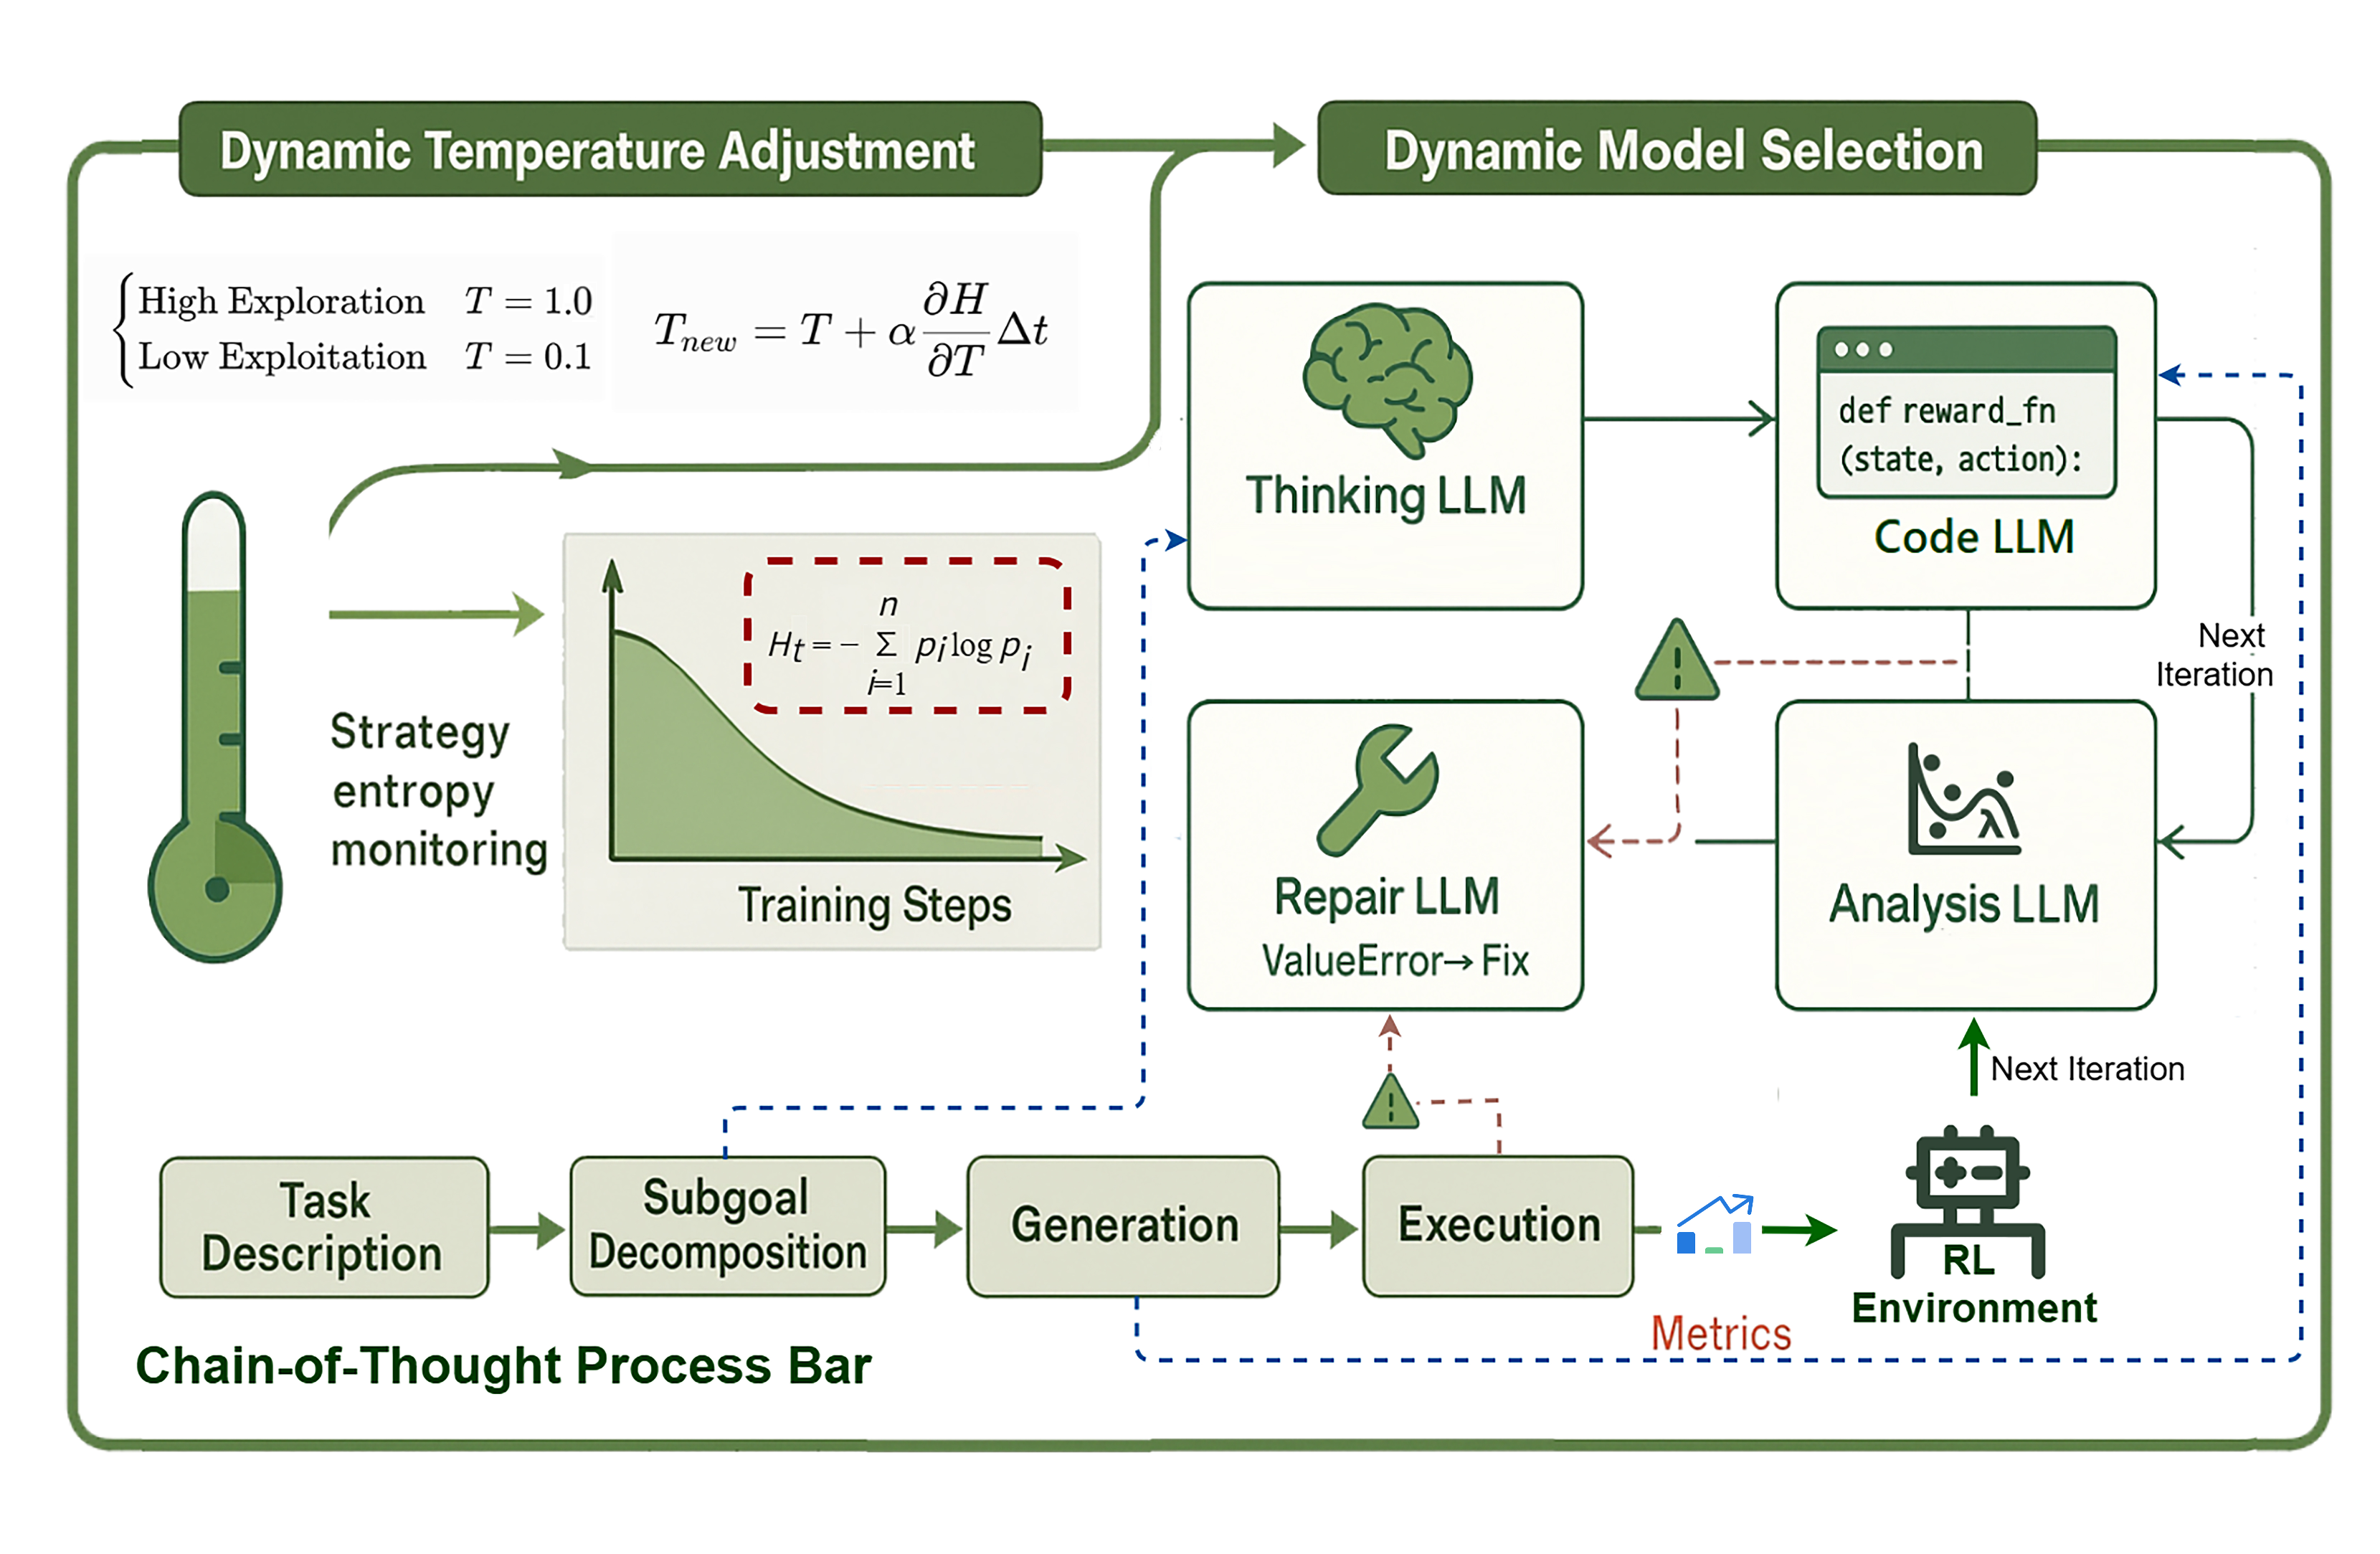
\includegraphics[width=0.95\linewidth]{Figures/dual_6.pdf}
    \caption{DyCoT-RE control flow integrating temperature modulation and model selection within CoT iterative reasoning.}
    \label{fig:control-flow}
\end{figure*}

\subsubsection{Dynamic Temperature Adjustment}

Temperature adjustment modulates the sampling temperature $T$ 
based on policy entropy $H$, confidence $C$, and performance $R$. 
Entropy reflects generative diversity, confidence measures output stability, 
and performance evaluates reward improvement relative to historical best.

The update rule is formulated as:

\begin{equation}
T_{k+1}
=
\text{clip}
\left(
T_k
+
\alpha \frac{\partial T}{\partial H_k} \Delta t
\right),
\end{equation}

where $\alpha$ is a learning rate,
and the gradient $\frac{\partial T}{\partial H_k}$ reflects entropy-driven adjustment.
An alternative implementation combines smoothing and multiplicative adjustment:

\begin{equation}
T_{k+1}
=
\text{clip}
\left(
\alpha T_k
+
(1-\alpha) T_k f(H_k,C_k,R_k)
\right).
\end{equation}

Here, $f(H,C,R)$ integrates:

\begin{equation}
f(H,C,R)
=
f_R(R)
f_H(H)
f_C(C),
\end{equation}

where $f_R$ ensures performance protection, $f_H$ regulates entropy bounds,
and $f_C$ maintains confidence stability.

\subsubsection{Dynamic Model Selection}

Dynamic model selection adaptively routes sub-tasks to specialized LLMs, 
leveraging their complementary strengths across the reward engineering pipeline.

The four LLM classes include:
$\mathcal{M}_{\text{think}}$ for task understanding and semantic decomposition, 
$\mathcal{M}_{\text{code}}$ for reward function synthesis, 
$\mathcal{M}_{\text{repair}}$ for code correction, 
and $\mathcal{M}_{\text{analysis}}$ for performance evaluation and sub-reward weight updates.

Formally, the decomposition and generation process can be expressed as:

\begin{equation}
g_i = \mathcal{M}_{\text{think}}(S, C, D, E), 
\end{equation}

\begin{equation}
r_i(s,a) = \mathcal{M}_{\text{code}}(g_i, C), 
\end{equation}

\begin{equation}
w_i^{(t+1)} = \mathcal{M}_{\text{analysis}}(w_i^{(t)}, \text{fitness}^{(t)}, \{r_j^{(t)}\}), 
\end{equation}

Repair LLM intervenes when $\mathcal{M}_{\text{code}}$ outputs execution errors during evaluation.

Model selection at iteration $k$ follows:

\begin{equation}
    M_{k+1} =
    \begin{cases}
    \displaystyle
    \arg\max_{m \in \mathcal{M}_s} \text{Perf}(m), & 1-\epsilon, \\[8pt]
    \text{Random}(\mathcal{M}_s \setminus \{M_k\}), & \epsilon,
    \end{cases}
    \end{equation}
    

where $\mathcal{M}_s$ is the model pool for stage $s$, 
$\text{Perf}(m)$ the performance score, 
and $\epsilon$ the exploration rate ensuring selection diversity.

At each iteration, the next model $M_{k+1}$ is selected from pool $\mathcal{M}_s$ using epsilon-greedy selection,
where the highest-performing model is chosen with probability $1-\epsilon$ and a random model with probability $\epsilon$.
The pool includes a Repair LLM for error correction during reward code evaluation.

\subsubsection{Joint Adaptive Optimization}

Temperature adjustment and model selection operate as coordinated mechanisms within the optimization loop. Temperature $\tau$ influences the sampling distribution of reward candidates:
\begin{equation} 
r_i(s,a) \sim p(r_i | g_i, \tau), 
\end{equation}
where $g_i$ represents the subgoal specification from $\mathcal{M}_{\text{think}}$. This sampling process modulates exploration patterns in the reward space.

The joint objective combines both mechanisms:
\begin{equation} 
(\tau^*, M^*) = \arg\max_{\tau,M} \mathbb{E}_{\pi_\theta} \left[ \sum_{t=0}^{H} \gamma^t R_{\tau,M}(s_t,a_t) \right], 
\end{equation}
where $R_{\tau,M}(s,a)$ denotes the reward function generated under temperature $\tau$ and model configuration $M$, and $H$ represents the episode horizon.


\section{Experiments}


\subsection{Experimental Setup}


DyCoT-RE is evaluated on four reinforcement learning environments,
which span diverse task difficulties, action spaces, and complexity levels.
Standard benchmarks include CartPole, BipedalWalker, and Ant,
covering discrete control tasks and high-dimensional continuous locomotion.

To assess performance on novel environments beyond pretrained knowledge, we introduce SpaceMining,
a custom environment with multi-objective resource collection and dynamic energy constraints.
Unlike standard environments that LLMs may encounter during pretraining, 
SpaceMining tests whether reward design can succeed through task understanding rather than prior knowledge.

\subsubsection{Baselines and Comparison Strategies}

We evaluate DyCoT-RE against two primary baselines:

(1) Human-designed rewards: Manually crafted reward functions from standard Gymnasium\cite{towers2024gymnasiumstandardinterfacereinforcement} 
implementations for CartPole, BipedalWalker, and Ant. For SpaceMining, we design corresponding reward functions following similar principles.

(2) Eureka: 
An established LLM-based framework for automated reward synthesis that employs iterative code generation and performance-based selection. 
We adapt its pipeline to Gymnasium-based evaluations for fair comparison.

\subsubsection{Ablation Comparisons}  

To evaluate individual contributions within DyCoT-RE, we include the following controlled variants:

- Zero-shot reward generation: Reward generation using direct prompts without CoT reasoning.

- Static temperature: Sampling temperature remains fixed throughout training. 

- Single model: A single LLM handles all reward generation tasks without dynamic model selection.

These comparisons isolate the contributions of CoT-based reasoning and the dual-dynamic mechanisms.




\subsubsection{Implementation Details}


We evaluate DyCoT-RE on three environments from the Gymnasium suite — CartPole-v1\footnote{\url{https://gymnasium.farama.org/environments/classic_control/cart_pole/}}, BipedalWalker-v3\footnote{\url{https://gymnasium.farama.org/environments/box2d/bipedal_walker/}}, and Ant-v5\footnote{\url{https://gymnasium.farama.org/environments/mujoco/ant/}}—alongside a custom-designed SpaceMining environment for evaluating performance in unseen domains.

All experiments use Proximal Policy Optimization (PPO) from Stable-Baselines3 with Adam optimizer, learning rate of 3e-4, batch size 64, GAE parameter $\lambda=0.95$, and discount factor $\gamma=0.999$.

DyCoT-RE generates reward functions using local LLMs served via Ollama, sampling eight reward candidates in parallel at each CoT iteration.

Final performance metrics are computed as the mean over ten test episodes with different random seeds.

\begin{table}[ht]
    \centering
    \scriptsize % 小字号
    \setlength{\tabcolsep}{4pt} % 紧凑列间距
\scriptsize
\caption{Task specifications for evaluated RL environments.}
\label{tab:env_specs}
\begin{tabular}{lccc}
\toprule
Environment & State/Action Dims & Episode Steps \\
\midrule
CartPole-v1 & 4 / 1 discrete & 500 \\
BipedalWalker-v3 & 24 / 4 continuous & 1600 \\
Ant-v5 & 111 / 8 continuous & 1600 \\
SpaceMining & 53 / 3 continuous & 1200 \\
\bottomrule
\end{tabular}
\end{table}





\subsection{Performance Across Environments} 

We compare DyCoT-RE against Human-designed and Eureka baselines across all evaluated environments. 
Figure~\ref{fig:bar_comparison} shows that DyCoT-RE achieves higher average rewards in all tested scenarios, with performance gaps increasing as task complexity grows.

\begin{figure}[ht]
\centering
\includegraphics[width=0.9\linewidth]{Figures/bar_comparison_8.pdf}
\caption{Final average rewards across environments: DyCoT-RE (blue), Eureka (light grass), and Human-designed (dark grass).}
\label{fig:bar_comparison}
\end{figure}

Figure~\ref{fig:learning_curves} provides insights into the learning dynamics. 
In CartPole, all methods converge quickly due to low-dimensional discrete dynamics, though DyCoT-RE converges slightly faster convergence. 
In BipedalWalker, DyCoT-RE exhibits a two-phase pattern: initial exploration volatility followed by stable growth and smoother long-term convergence. 
In the Ant environment, all methods initially encounter performance valleys, but DyCoT-RE recovers more quickly and achieves sustained improvement to higher fitness scores, while Eureka shows instability throughout training.
In SpaceMining, DyCoT-RE maintains steady progress while baselines show flat or unstable performance, demonstrating effective generalization to novel tasks.

\begin{figure}[ht]
\centering
\includegraphics[width=0.9\linewidth]{Figures/reward_episode_curve_8.pdf}
\caption{Learning curves across environments. DyCoT-RE exhibits consistent advantages in stability and long-term reward growth, especially in complex settings.}
\label{fig:learning_curves}
\end{figure}

Table~\ref{tab:perf_summary} compares performance across four tasks using three metrics: 
Sample Efficiency measures the number of timesteps required to reach a threshold reward, defined as 80\% of the task-specific maximum score. 
Success Rate indicates the proportion of runs that eventually exceed this threshold. 
Late Gain quantifies the reward improvement from the early performance plateau to the final evaluation, reflecting long-term optimization potential.


\begin{table}[ht]
\centering
\scriptsize
\setlength{\tabcolsep}{4pt}
\caption{Cross-task performance comparison.
\colorbox{skyblue!15}{Blue}: the best value per column, 
\colorbox{grass!15}{green}: the second-best. 
Success Rate is omitted for Human due to deterministic reward completion.}
\label{tab:perf_summary}
\begin{tabular}{llccc}
\toprule
Task & Method & Sample Eff. $\downarrow$ & Succ. Rate $\uparrow$ & Late Gain $\uparrow$ \\
\midrule

\multirow{3}{*}{CartPole} 
& {DyCoT-RE} & \cellcolor{skyblue!15}75k & \cellcolor{skyblue!15}98\% & \cellcolor{skyblue!15}450 \\
& {Eureka} & \cellcolor{grass!15}115k & \cellcolor{grass!15}95\% & \cellcolor{grass!15}440 \\
& Human & 286k & -- & 400 \\

\midrule

\multirow{3}{*}{BipedalWalker} 
& {DyCoT-RE} & \cellcolor{skyblue!15}393k & \cellcolor{skyblue!15}92\% & \cellcolor{skyblue!15}387 \\
& {Eureka} & \cellcolor{grass!15}428k & \cellcolor{grass!15}83\% & \cellcolor{grass!15}366 \\
& Human & 720k & -- & 309 \\

\midrule

\multirow{3}{*}{Ant} 
& {DyCoT-RE} & \cellcolor{skyblue!15}16.19M & \cellcolor{skyblue!15}85\% & \cellcolor{skyblue!15}5398 \\
& {Eureka} & 21.53M & \cellcolor{grass!15}70\% & \cellcolor{grass!15}2412 \\
& Human & \cellcolor{grass!15}19.92M & -- & -240 \\

\midrule

\multirow{3}{*}{SpaceMining} 
& {DyCoT-RE} & \cellcolor{skyblue!15}1.31M & \cellcolor{skyblue!15}80\% & \cellcolor{skyblue!15}2285 \\
& {Eureka} & 1.74M & \cellcolor{grass!15}65\% & 189 \\
& Human & \cellcolor{grass!15}1.56M & -- & \cellcolor{grass!15}1230 \\

\bottomrule
\end{tabular}
\end{table}

DyCoT-RE outperforms baselines across all evaluated metrics: 
it reaches target performance faster, succeeds more reliably, and continues improving in later training stages. 
These advantages are most evident in high-dimensional environments, where static reward design approaches show limited adaptability.

\subsection{Ablation Study}
\label{sec:ablation}

This section conducts an ablation study to examine the individual contribution of each component in DyCoT-RE, including CoT reasoning, temperature adjustment, and model selection, as well as their combined synergistic effects.

\subsubsection{Impact of CoT Reasoning}


We evaluate the impact of incorporating CoT reasoning into reward engineering by comparing DyCoT-RE's CoT-enabled variant against a zero-shot baseline lacking structured intermediate reasoning.



Figure~\ref{fig:cot_ablation} summarizes reward distributions for both methods across the four benchmark environments. A consistent pattern emerges: CoT-enabled rewards exhibit higher means, lower variance, and reduced outlier incidence compared to zero-shot. In CartPole and SpaceMining, CoT-enabled results are tightly clustered near the environment's upper performance bounds, whereas zero-shot results are widely dispersed, with a substantial proportion of runs yielding suboptimal or even near-zero rewards. This reflects CoT's ability to systematically decompose task objectives into interpretable sub-rewards, enhancing sample efficiency and stabilizing policy learning.



\begin{figure}[ht]
    \centering
    \includegraphics[width=1.0\textwidth]{Figures/cot_ablation_4.pdf}
    \caption{Final reward distributions for CoT-enabled vs zero-shot reward generation across environments.}
    \label{fig:cot_ablation}
    \end{figure}

    In BipedalWalker, a notable deviation is observed. CoT-enabled runs yield a concentrated reward range between 250 and 310, with virtually no severely negative outcomes. In contrast, the zero-shot condition presents a clear bimodal distribution: one cluster achieves moderate reward levels around 150 to 250, while the other collapses into strongly negative regimes. This instability reflects the inability of zero-shot reward generation to encode essential gait balance or locomotion constraints, often resulting in policy failure.

    In Ant, zero-shot results are narrowly concentrated near baseline values associated with default movement penalties. This indicates that while these reward functions do not collapse, they lack task-driving gradients for effective behavior shaping. In contrast, CoT-based rewards achieve a wider spread toward higher values, reflecting meaningful progress and more informative optimization signals.
    

Taken together, these results illustrate that CoT reasoning reliably improves reward interpretability and training stability, especially in settings with complex objectives.

    


\subsubsection{Impact of Temperature Adjustment}


Due to computational constraints and consistent observed trends across environments, 
temperature adjustment and model selection ablation were conducted on BipedalWalker as a representative continuous control task, 
while CoT reasoning was evaluated on all four environments to confirm its general effectiveness.

This section investigates the effect of temperature settings by sweeping $T \in [0.0, 1.0]$ on the BipedalWalker environment. 

Table~\ref{tab:temp_sweep} reports BipedalWalker results under different temperature settings, including average and maximum fitness, standard deviation, and reward efficiency ratio. DyCoT-RE achieves the best performance across all metrics, with a large margin in efficiency ratio due to its high average fitness and low variability. 
Among fixed-temperature settings, moderate values (0.4–0.6) deliver relatively strong results, yet still fall short of DyCoT-RE.

\begin{table}[ht]
\centering
\scriptsize % 小字号
\setlength{\tabcolsep}{4pt} % 紧凑列间距
\caption{BipedalWalker performance under different temperature settings. \colorbox{skyblue!15}{Blue}: the best value per column, 
\colorbox{grass!25}{green}: the second-best, \colorbox{grass!15}{green}: the third-best }
\label{tab:temp_sweep}
\begin{tabular}{c|c|c|c|c}
\hline
Temp & Avg Fit$\uparrow$ & Max Fit $\uparrow$& Std$\downarrow$  & Eff. Ratio$\uparrow$ \\
\hline
0.0 & 81.93 & 301.15 & 148.67 & 0.55 \\
0.1 & 149.56 & 310.94 & 155.22 & 0.96 \\
0.2 & 242.74 & \cellcolor{grass!25}313.60 & 125.47 & 1.93 \\
0.3 & 210.07 & 311.17 & 140.49 & 1.50 \\
0.4 & \cellcolor{grass!15}244.19 & 311.94 & \cellcolor{grass!25}107.02 & \cellcolor{grass!25}2.28 \\
0.5 & 215.84 & 310.69 & 131.01 & 1.65 \\
0.6 & \cellcolor{grass!25}248.11 & \cellcolor{grass!15}312.48 & \cellcolor{grass!15}120.45 & \cellcolor{grass!15}2.06 \\
0.7 & 225.88 & 312.42 & 131.43 & 1.72 \\
0.8 & 74.33 & 310.42 & 143.91 & 0.52 \\
0.9 & 145.02 & 310.02 & 148.51 & 0.98 \\
1.0 & 192.38 & 310.40 & 138.37 & 1.39 \\
\rowcolor{skyblue!15}
DyCoT-RE & 292.8 & 315.6/87.2 & 55.2 & 5.30 \\
\hline
\end{tabular}
\end{table}

Static sweeps show that mid-range temperatures yield higher fitness and lower variance than extremes. 
DyCoT-RE’s dynamic temperature regulation consistently outperforms these static settings, 
adapting temperature during training to maintain an effective exploration-exploitation trade-off. 


\subsubsection{Impact of Model Selection}

Finally, we evaluate the impact of DyCoT-RE's dynamic model selection by comparing it against individual static LLM baselines on the BipedalWalker environment. 
Table~\ref{tab:model_selection} compares different LLM backends on BipedalWalker in terms of average fitness, peak performance, stability, and reward efficiency. 

DyCoT-RE achieves the highest average fitness with exceptionally low standard deviation and the best efficiency ratio, demonstrating its capability to consistently generate high-quality rewards across diverse sub-tasks. 

In contrast, while codegemma achieves competitive performance, its higher standard deviation results in a substantially lower efficiency ratio, indicating reduced stability and generalizability compared to DyCoT-RE.

\begin{table}[ht]
\centering
\scriptsize % 小字号
\setlength{\tabcolsep}{4pt} % 紧凑列间距
\caption{Performance comparison of different LLM backends (N=20) in BipedalWalker. \colorbox{skyblue!15}{Blue}: the best value per column, 
\colorbox{grass!25}{green}: the second-best}
\label{tab:model_selection}
\begin{tabular}{l|c|c|c|c}
\hline
Model (size) & Avg Fit $\uparrow$ & Max Fit $\uparrow$ & Std $\downarrow$ & Eff. Ratio $\uparrow$ \\
\hline
codegemma (7b) & 260.8 & 301.8 & \cellcolor{grass!25}34.2 & 3.46\cellcolor{grass!25} \\
codeqwen (7b) & 32.6 & 307.6 & 98.42 & 0.33 \\
deepseek-coder (6.7b) & -4.5 & 295.3 & 98.19 & -0.05 \\
deepseek-r1 (8b) & 44.6 & \cellcolor{skyblue!25}321.2 & 122.07 & 0.37 \\
gemma3 (4b) & \cellcolor{grass!25}278.0 & 314.8 & 142.04 & 3.39 \\
llama3.1 (8b) & 162.2 & 318.4 & 150.75 & 1.08 \\
qwen2.5 (7b) & 177.0 & 319.5 & 151.51 & 1.17 \\
qwen2.5-coder (7b) & 125.6 & 313.7 & 163.16 & 0.77 \\
DyCoT-RE & \cellcolor{skyblue!25}297.28 & \cellcolor{grass!25}316.57 & \cellcolor{skyblue!25}89.47 & \cellcolor{skyblue!25}6.46 \\
\hline
\end{tabular}
\end{table}

While individual models occasionally excel on specific tasks, DyCoT-RE’s dynamic model routing achieves broadly consistent performance, 
balancing reward quality and stability in complex continuous control environments.

In summary, the ablation study indicates that each module—CoT reasoning, temperature adjustment, and model selection—plays a substantive role in enhancing DyCoT-RE’s performance.

\subsection{DyCoT-RE in SpaceMining: Results in an LLM-Unseen Environment}
\label{sec:space_mining_analysis}

To evaluate DyCoT-RE in an out-of-distribution scenario without task-specific priors, we constructed the SpaceMining environment—a multi-objective domain involving dynamic hazards and energy constraints. This setting challenges the model to formulate effective rewards from natural language alone, testing its semantic generalization and reasoning capabilities.

\begin{figure}[ht]
\centering
\includegraphics[width=\linewidth]{Figures/reward_energy_curves.pdf}
\caption{Training dynamics in SpaceMining. Left: reward and fitness improve steadily, showing effective long-term optimization. Right: stable energy levels and growing inventory indicate successful energy-resource balancing.}
\label{fig:space_mining_curves}
\end{figure}



Figure~\ref{fig:space_mining_curves} illustrates the learning trajectory of DyCoT-RE. 
From early-stage exploration to late-stage optimization, we observe concurrent increases in reward and fitness, 
with consistent energy regulation and inventory accumulation. 
These trends reflect reward structures that incentivize planning, efficiency, and safe behavior.


\begin{figure}[ht]
\centering
\includegraphics[width=0.95\linewidth]{Figures/correlation_heatmap.pdf}
\caption{
    The evolution of normalized reward component contributions in DyCoT-RE for SpaceMining}
\label{fig:component_evolution}
\end{figure}

Figure~\ref{fig:component_evolution} shows the relative contribution of each reward component during 
training iterations. Positive and negative values indicate reinforcement and penalty signals respectively, 
while zero values with reduced opacity show inactive components. Border colours denote component lifecycle 
stages including new, maintained, core, and deprecated components, with column labels showing corresponding 
fitness scores. 
Component contribution is computed as $\text{Contr}_i = \frac{\overline{r_i}}{\sum_j \overline{r_j}} \times 100\%$, 
where $\overline{r_i}$ is the average reward from component $i$.

The system begins with a minimal setup focused on mining progress, distance penalties, and energy tracking. 
As training proceeds, DyCoT introduces new components such as obstacle avoidance in Iteration 3, inventory-based delivery efficiency in Iteration 5, and asteroid discovery incentives in Iteration 7. 
These additions are not arbitrary but driven by observed performance shifts. 
For instance, after dynamic obstacle handling is introduced, the agent’s survival rate improves significantly. 
Conversely, some components such as velocity control lose their relevance and are phased out by Iteration 3, as their function becomes redundant once obstacle-aware navigation is in place. 
The energy management module, on the other hand, steadily increases in importance and becomes a core contributor throughout the later iterations. 
This dynamic component lifecycle—characterized by incremental expansion, adaptive weighting, and timely deprecation—demonstrates DyCoT’s capacity for modular, interpretable, and performance-aligned reward optimization.


\begin{table}[ht]
    \centering
    \scriptsize % 小字号
    \setlength{\tabcolsep}{4pt} % 紧凑列间距
    \caption{DyCoT Strategy Metrics Across Iterative Architectures. 
    \colorbox{skyblue!15}{Blue}: the best value per column, 
\colorbox{grass!25}{green}: the second-best.}
    \label{tab:dycot_dynamics_full}
    \begin{tabular}{c|c|c|c|c|c}
    \toprule
    Iter & Temperature & Entropy & Confidence & Best Reward & Reward Gain (\%) \\
    \midrule
    0 & 0.800 & 0.912 & 0.642 & 880.2 & -- \\
    1 & 0.700 & 0.946 & 0.705 & 1124.4 & \cellcolor{grass!25}+27.7 \\
    2 & 0.669 & 0.928 & 0.748 & 1320.3 & +17.4 \\
    3 & 0.639 & \cellcolor{skyblue!15}0.986 & 0.778 & 3475.5 & \cellcolor{skyblue!15}+163.2 \\
    4 & 0.600 & 0.934 & 0.791 & 3551.0 & +2.2 \\
    5 & 0.556 & 0.914 & 0.807 & 3801.3 & +7.0 \\
    6 & \cellcolor{grass!25}0.534 & 0.962 & \cellcolor{grass!25}0.815 & \cellcolor{grass!25}3876.2 & +2.0 \\
    7 & \cellcolor{skyblue!15}0.517 & \cellcolor{grass!25}0.972 & \cellcolor{skyblue!15}0.824 & \cellcolor{skyblue!15}4003.2 & +3.3 \\
    \bottomrule
    \end{tabular}
    \end{table}
    
    Table~\ref{tab:dycot_dynamics_full} illustrates the evolution of key strategy-level metrics throughout all DyCoT iterations. As the architecture matures from Iteration 0 to 7, we observe a consistent decline in sampling temperature, indicating increased confidence in policy generation. Entropy fluctuates with architecture changes, notably peaking at Iteration 3 when major reward components are introduced. Confidence improves steadily, rising from 0.64 to 0.82, in parallel with fitness gains. Reward gain is computed relative to the previous iteration, with Iteration 3 marking a significant performance inflection point. 
    Subsequent gains are more incremental, reflecting architectural stabilization.


In summary, DyCoT-RE exhibits the capacity for iterative reward adaptation. It evolves from simple distance-based signals to structured reward components that support coordinated behaviors such as exploration, energy regulation, and goal-oriented progression—achieving consistent performance in environments with minimal prior knowledge.

\section{Discussion}

This work presents DyCoT-RE, a reward engineering framework that integrates CoT reasoning with dual-dynamic optimization strategies for automated reward function design. Our experimental evaluation across four RL environments demonstrates consistent performance improvements over human-designed rewards and existing automated baselines, with the most significant gains observed in complex, multi-objective environments.


Three findings emerge from our evaluation. First, CoT decomposition improves reward interpretability and stability by breaking complex objectives into manageable components. 
Second, dynamic strategies outperform static configurations: adaptive temperature control balances exploration-exploitation better than fixed settings, while model selection leverages diverse LLM strengths for higher performance and consistency. 
Third, SpaceMining results demonstrate DyCoT-RE's ability to generate effective reward functions even in unfamiliar environments, suggesting that structured reasoning can compensate for the absence of domain-specific priors.

DyCoT-RE introduces computational overhead and depends on underlying LLM capabilities. Evaluation is limited to four environments, and the framework uses general-purpose models not optimized for reward engineering. 
Future research could explore specialized models fine-tuned for reward engineering, incorporate multi-modal inputs beyond natural language, expand evaluation to broader environment categories, and develop transfer learning mechanisms to leverage successful reward designs across similar domains.

DyCoT-RE demonstrates that combining structured reasoning with adaptive optimization offers a promising direction for scalable automated reward engineering, particularly in complex RL domains where traditional approaches prove insufficient.

\section{Conclusion}

This paper introduces DyCoT-RE, a framework that addresses the challenge of automated reward function design in RL. 
The main contribution lies in combining structured reasoning through CoT prompting with adaptive optimization mechanisms that dynamically adjust both temperature and model selection throughout the reward engineering process.

Evaluation demonstrates that DyCoT-RE consistently produces effective and stable reward functions across tasks ranging from simple control to complex, 
multi-objective scenarios, including a novel environment unfamiliar to LLMs.
The results highlight its potential as a scalable solution for RL tasks requiring structured and evolving reward design 
for complex objectives.

\bibliography{adaptive_cot_reward_rl} 

\end{document}
